\section{Applications}

\subsection{Thin parts}
\begin{itemize}
\item Casings (e.g. for electronics)
\item Prototypes for blowmold parts or sheet metal parts etc.
\item Miniature models, architectural models
\item Microstructures
\item Lithophanes
\end{itemize}

Show the effect of the planned toolpath on the performance of varying thickness microstructures.
Compare to \cite{bates2018compressive}.


\begin{figure*}
\centering
\setlength{\figwidth}{0.1\textwidth}
\setlength{\figheight}{0.1\textwidth}
\begin{subfigure}{\figwidth}\centering
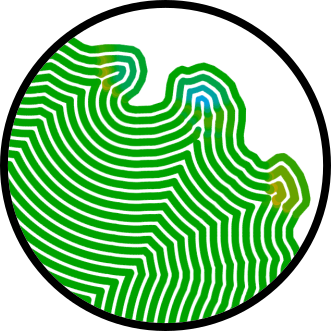
\includegraphics[height=\figheight]{sources/applications/david.png}
\caption{Statue}%label{applications_}
\end{subfigure}
\begin{subfigure}{\figwidth}\centering
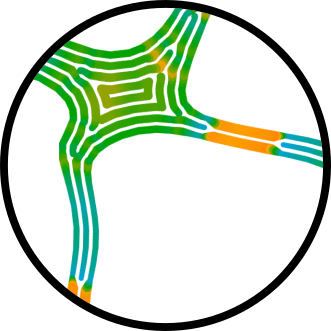
\includegraphics[height=\figheight]{sources/applications/gyroid.png}
\caption{Gyroid}%label{applications_}
\end{subfigure}
\begin{subfigure}{\figwidth}\centering
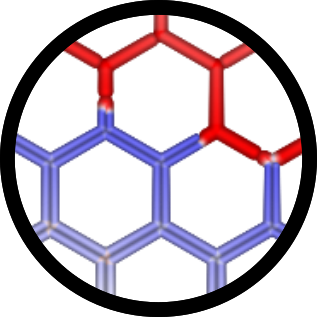
\includegraphics[height=\figheight]{sources/applications/hex_grid.png}
\caption{Hex}%label{applications_}
\end{subfigure}
\begin{subfigure}{\figwidth}\centering
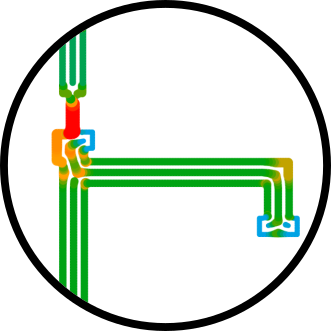
\includegraphics[height=\figheight]{sources/applications/house.png}
\caption{House}%label{applications_}
\end{subfigure}
\begin{subfigure}{\figwidth}\centering
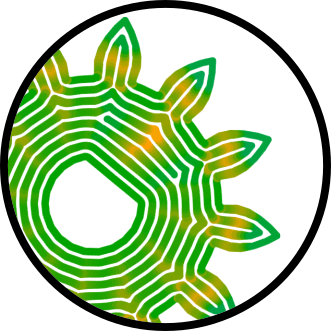
\includegraphics[height=\figheight]{sources/applications/pinion_gear_motor.png}
\caption{Gear}\label{applications_gear}
\end{subfigure}
\begin{subfigure}{\figwidth}\centering
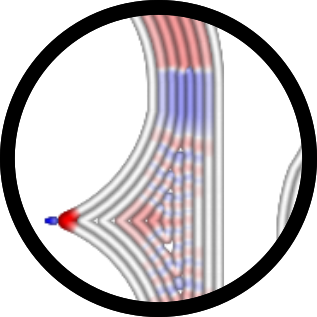
\includegraphics[height=\figheight]{sources/applications/pocket_operator_case.png}
\caption{Case}%label{applications_}
\end{subfigure}
\begin{subfigure}{\figwidth}\centering
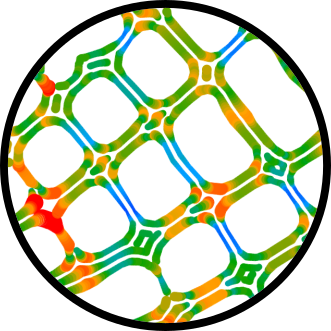
\includegraphics[height=\figheight]{sources/applications/topopt_bone.png}
\caption{Bone}%label{applications_}
\end{subfigure}
\begin{subfigure}{\figwidth}\centering

\includegraphics[height=\figheight]{sources/applications/tud_logo.png}
\caption{TUD}%label{applications_}
\end{subfigure}
\begin{subfigure}{\figwidth}\centering

\includegraphics[height=\figheight]{sources/applications/ultimaker_logo.png}
\caption{UM}%label{applications_}
\end{subfigure}
\caption{
Closeups of results for the inward distributed beading strategy for various applications.
The extrusion widths are visualized exaggeratedly and using a color scheme exaplained in \cref{visualized_accuracy}.
}
\label{application_closeups}
\end{figure*}


\begin{figure}
\centering
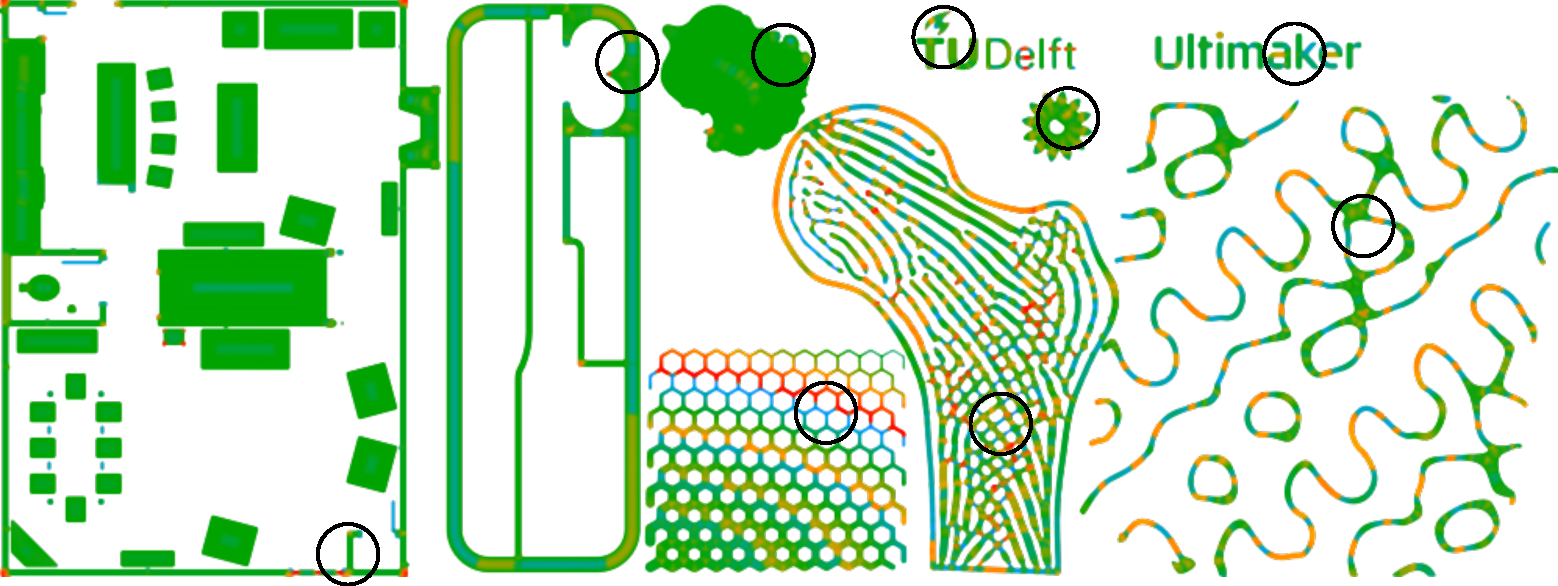
\includegraphics[width=\columnwidth]{sources/applications/combined_small_dilated_circled.pdf}
\caption{
Visualization of the widths for the output toolpaths of the inward distributed beading strategy applied to various example application objects.
A legend for the colors can be found in \cref{visualized_accuracy}.
From left to right and top to bottom: a house, a case for electronics, a statue, two common logos, a gear, a topologically optimized bone structure, a homogeneous lateral thickness tilted gyroid structure and a heterogeneous thickness hexagonal grid.
}
\label{applications_overview}
\end{figure}


\begin{figure}
\centering
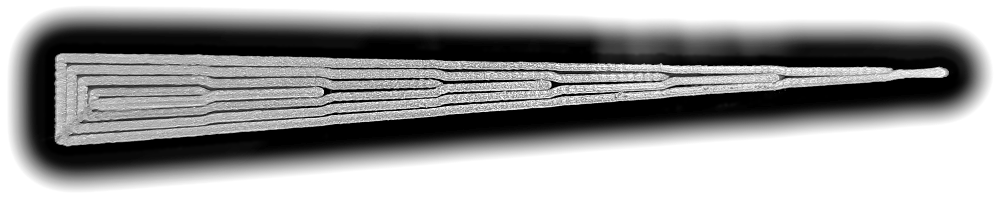
\includegraphics[width=\columnwidth]{sources/applications/wedge_print_v2.png}
\caption{
A small wedge shape printed using the variable width scheme prescribed by the ditributed beading strategy.
}
\label{wedge_print}
\end{figure}


\subsection{Widening}
Regions where the model is narrower than the nozzle size can be printed with a bead width larger than the model thickness.